\chapter{Fähigkeiten}
Skillsystem, Lehrer
Leveln
\begin{itemize}
	\item Idee für Erweiterung des Soldaten-Regenerationsskills: ein Punkt kann sein, dass er gelernt hat, sein Essen bedachter zu verspeisen und besser zu verwerten. Das führt zu einer Erhöhung der Heilung pro Sekunde
\end{itemize}

\section{Leveln}
\begin{itemize}
	\item Es gibt verschiedene Arten von Skills. Manche können erlernt und etwas gesteigert werden, ohne dass dafür besondere Dinge oder Zeit nötig sind (zB Regeneration). Die anderen wiederum haben ein bestimmtes System aus Selbst-Lernen, Lehrmeistern und Üben
	\item Ich erkläre das System am Beispiel des Schlösserknackens unter der Annahme, dass wir 5 Stufen der Beherrschung eines Skills einführen (zB Neuling, Lehrling, Adept, Meister, Großmeister)
	\item Zu Beginn hat man die Fähigkeit nicht. Es gibt nun zwei Wege, sie zu erwerben:\\
	1. Selbstlehrend. Dabei setzt man sich einfach mal an ein zu knackendes Schloss und egal ob man es schafft oder nicht, man ist nun in der ersten Stufe, Neuling. \\
	2. Lehrmeister. Man kann auch zu einem entsprechenden Lehrmeister gehen (z.B. ein Schlosser) und ihn bitten, einem die Grundlagen beizubringen.
	\item um nun die Fähigkeit zu verbessern sind zwei Abschnitte relevant: Das Üben und der Aufstieg in die nächste Stufe (und damit verbunden neue Fähigkeiten-Möglichkeiten)
	\item erstmal zum Aufstieg. Um die nächste Stufe zu erreichen, ist IMMER ein Lehrmeister (oder auf den niedrigen Stufen meinetwegen auch Lehrbücher) nötig. Dies sorgt auch dafür, dass wir die Relevanz von Geld in unserem Spiel erhöhen.
	In unserem Beispiel würde einem der Schlosser Erläuterungen zu kompizierteren Schlössern geben und sie zeigen.
	\item das Üben ist nötig, bevor man aufsteigen darf. Denn nur, weil ich die Grundschule geschafft habe, heißt das nicht, dass ich bereit für den Master bin. Keiner kann als Kind direkt nach der Erklärung zum Fahrradfahren losradeln und fährt nicht in den nächsten Baum oder kippt um.
	Üben beideutet die Anwendung des Skills in Ausreichender Menge oder Zeit für das Erreichen der kommenden Stufe. Das muss im Allgemeinen während des Spiels erfolgen. Allerdings können da die Lehrmeister - eingeschränkt - helfen. So könnte einem der Schlosser ein paar alte oder falsche oder einfach Übungsschlösser zur Verfügung stellen, damit man an ihnen üben kann. Das kostet natürlich. Macht man dieses Üben unter Aufsicht eines Meisters, dann kommt man schneller voran (man muss zB nicht 20 sondern nur 10 Schlösser knacken). ABER die Menge der Übung, die man bei einem Meister absolvieren kann, variiert je nach aktueller Stufe. So kann man im niedrigsten Bereich alle Übungseinheiten beim Meister absolvieren, doch will man Großmeister werden, dann vllt nur die ersten 20 Prozent...
	\item andere Skills wiederum gibt es nur in einer Steigerungsform: Man kann sie oder auch nicht und vielleicht kann man besser werden, aber nur in einem marginalen Rahmen und dann nur durch Anwendung (zB tanzen)
\end{itemize}

\section{Beispiel eines Fähigkeitenbaums}
\begin{figure}[h]
    \centering
    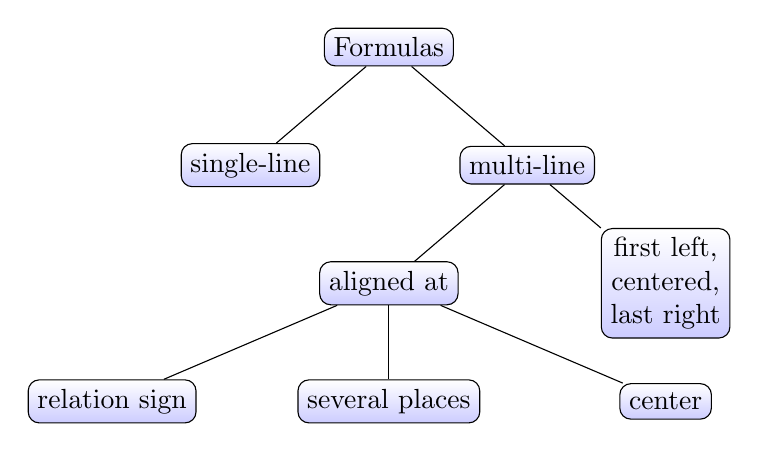
\begin{tikzpicture}[sibling distance=10em,
        every node/.style = {shape=rectangle, rounded corners,
            draw, align=center,
            top color=white, bottom color=blue!20}]]
        \node {Formulas}
        child { node {single-line} }
        child { node {multi-line}
            child { node {aligned at}
                child { node {relation sign} }
                child { node {several places} }
                child { node {center} } }
            child { node {first left,\\centered,\\last right} } };
    \end{tikzpicture}
    \caption{Fähigkeitenbaum Rhetorik}
    \label{fig:faehigkeitenbaum_rhetorik}
\end{figure}
